\section{Results and analysis}
\label{sec:analysis}

\subsection{Property distributions}
Here we will look at the frequency distributions (histograms) comparing the characteristics of CPSBs, RPSBs an their control galaxies.

The surface brightness profile of a galaxy is generally a function of radius from the nucleus. The rate of change of brightness can be described by the S\'ersic function or S\'ersic  index (SI). Low values of SI $\sim$1 relate to disc-type galaxies, whereas SI values of 3 or more are measured in galaxies with compact bright nuclei, indicative of more evolved systems.  

We compare the distributions of CPSBs with that of the RPSB sample in terms of S\'ersic index, stellar mass $M_*$, and redshift z. These distributions are taken from the data in Tables \ref{tab:my-CPSBs} and \ref{tab:my-RPSBs}. The frequency distribution histograms are plotted in Figures \ref{fig:Sersic-plot}, \ref{fig:stellar-mass-plot} and \ref{fig:redshift-plot} respectively.

The distribution of S\'ersic index values as shown in Figure \ref{fig:Sersic-plot} covers a wide range of values indicating a wide range of morphologies. CPSBs  generally have higher S\'ersic index values than RPBs. This suggests that CPBs tend to have concentrated nuclei and a spheroidal morphology contrary to the more disc-like RPSBs with lower SI-n values.

\begin{figure}
    \centering
    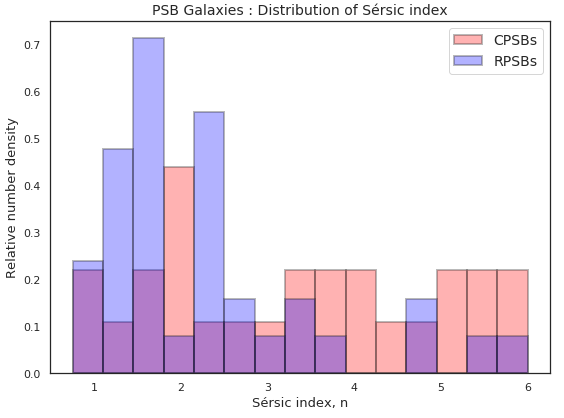
\includegraphics[width=\columnwidth]{images/JupyterPlots/Dist-Sersic-Index-All.png}
    \caption{Distribution of S\'ersic index (SI) values. The relative number density distribution of the S\'ersic index value for 26 CPSBs (red histogram) and 36 RPSBs (blue) are plotted. Five PSBs with unreliable SI values (SI = 6.000) in the NSA data  have been excluded.}
    \label{fig:Sersic-plot}
\end{figure}

\begin{figure}
    \centering
    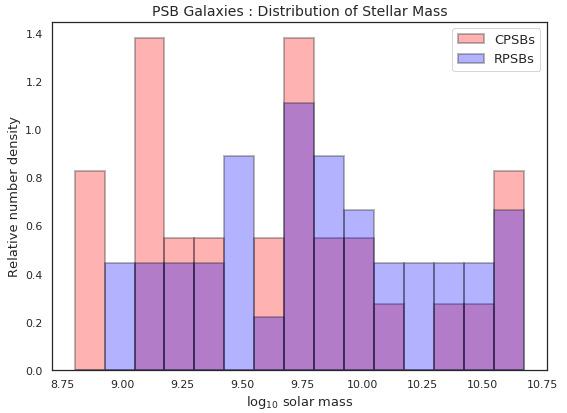
\includegraphics[width=\columnwidth]{images/JupyterPlots/Dist-Stellar-Mass-All.png}
    \caption{Distribution of Stellar mass of our sample of CPSBs (rad) and RPSBs (blue). On the scale of $\log_{10}$\Msun\ a fairly uniform distribution of stellar mass is apparent for both populations, CPSBs and RPSBs.}
    \label{fig:stellar-mass-plot}
\end{figure}

\begin{figure}
    \centering
    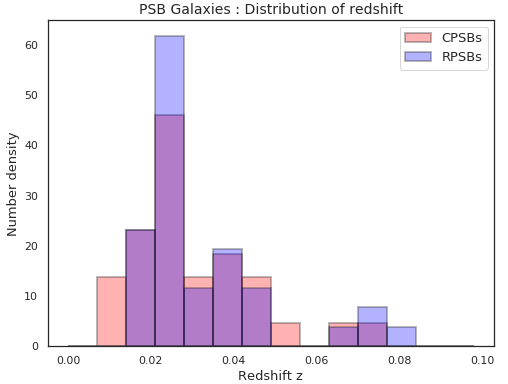
\includegraphics[width=\columnwidth]{images/JupyterPlots/Dist-z-All.png}
    \caption[PSB distribution in redshift]{Distribution in redshift: the redshift z as obtained from the NSA.Z data value for the CPSB sample (shaded in red) is compared to the RPSB sample (blue).}
    \label{fig:redshift-plot}
\end{figure}

\begin{figure}
    \centering
    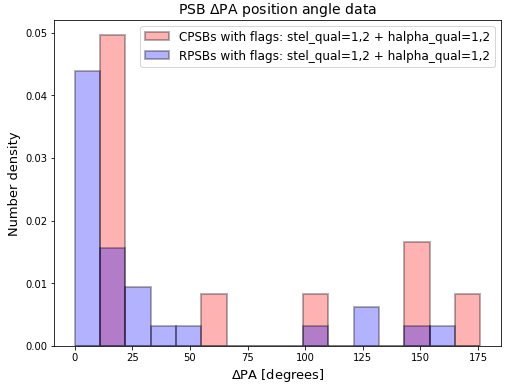
\includegraphics[width=\columnwidth]{images/JupyterPlots/Dist-Delta-PA-All-GoodFlags.png}
    \caption[Distribution of PSB velocity field position angles]{Distribution of PSB galaxy velocity map position angles for those PSBs with stellar velocity and gas velocity characteristics flagged as 'good' as denoted in the legend (details are provided in the text). CPSB PA density weights are plotted in red, RPSB PA weights in blue.}
    \label{fig:deltaPAdistribution}
\end{figure}

The velocity field position angle variance of the CPSB and PSB control galaxies is shown in Figure \ref{fig:controlDeltaPAs}. Both sets of control galaxies have low values of velocity field $\Delta$PAs, i.e. the stellar velocity and gas velocity fields are generally aligned.

\begin{figure}
    \centering
    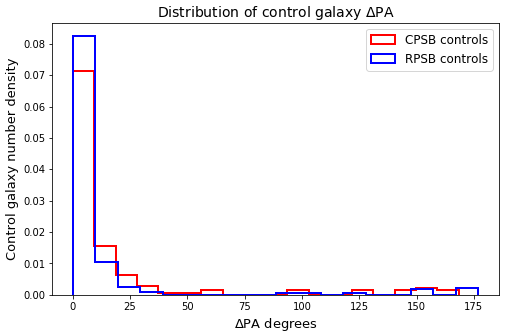
\includegraphics[width=\columnwidth]{images/JupyterPlots/Distribution-of-control-galaxy-deltaPA.png}
    \caption[Distribution of control galaxy $\Delta$PAs]{Distribution of control galaxy stellar and gas velocity field $\Delta$PAs.}
    \label{fig:controlDeltaPAs}
\end{figure}

\begin{figure}
    \centering
    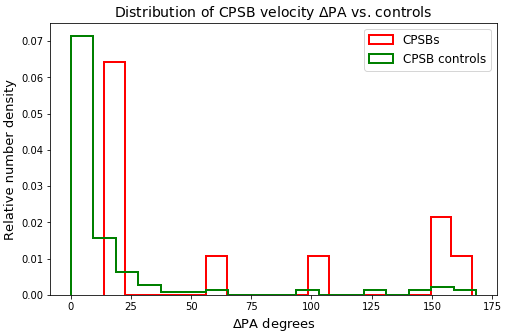
\includegraphics[width=\columnwidth]{images/JupyterPlots/Distribution-of-CPSB-dPA-vs-controls.png}
    \caption{Distribution of CPSB stellar-gas velocity $\Delta$PA vs. controls.}
    \label{fig:CPSBvsControlDeltaPAs}
\end{figure}

\begin{figure}
    \centering
    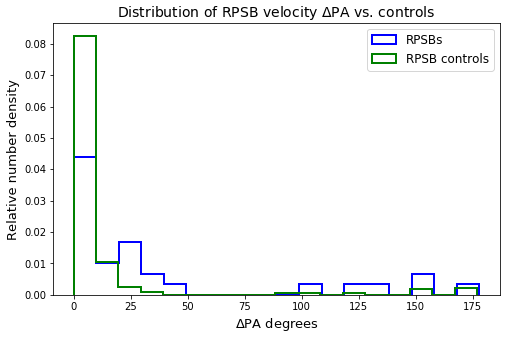
\includegraphics[width=\columnwidth]{images/JupyterPlots/Distribution-of-RPSB-dPA-vs-controls.png}
    \caption{Distribution of RPSB stellar-gas velocity $\Delta$PA vs. controls.}
    \label{fig:RPSBvsControlDeltaPAs}
\end{figure}

\subsection{The KS-test}
The Kolmogorov-Smirnov test: a statistical test to determine if two samples come from the same underlying distribution, see e.g. \citet{hodges1958significance}. We implement this test using the SciPy package \texttt{scipy.stats.kstest} module\footnote{\href{}{https://docs.scipy.org/doc/scipy/reference/generated/scipy.stats.ks\_2samp.html}}.

We ran the two-sided K-S test statistic on the distribution of $\Delta$ position angles obtained from the \texttt{kinemetry} analysis. The results are given in Table \ref{tab:K-S-tests}. The statistical significance inferred from the from the K-S test is that a high value of the test statistic, typically > 0.1, together with a low p-value, < 0.1 indicates that the samples are drawn from different statistical distributions. Here we note that the CPSB and RPSB samples originate from different distributions, and also each sample is from a different distribution from its corresponding control galaxy sample. The Python implementation \texttt{scipy.stats.ks\_2samp} accepts samples of different sizes.

\begin{table}
\caption[Kolmogorov-Smirnov statistical test]{Kolmogorov-Smirnov statistical test on various $\Delta$PA sample distributions. A high value of the K-S statistic > 10\%, together with a low p-value, < 10\% indicates that the samples come from different statistical distributions.}
\label{tab:K-S-tests}
\begin{tabular}{llcc}
\hline
$\Delta$PA sample 1  & $\Delta$PA sample 2 & K-S statistic & p-value \\
\hline
CPSB & RPSB & 0.467 & 0.040 \\
CPSB & CPSB controls & 0.755 & 0.000 \\
RPSB & RPSB controls & 0.520 & 0.000 \\
CPSB controls & RPSB controls & 0.197 & 0.001 \\
\hline
\end{tabular}
\end{table}

\subsection{Radon profile classification}
\label{sec:Radon-profile-classification}

A summary of the final visual classification method is shown in Table \ref{tab:Radon-class-summary}. The results of the Radon profile classification process for each of the individual target galaxies is provided in Appendix \ref{sec:visual-classification-tables}. 

\begin{table}
    \centering
    \caption{Summary of the classification of Radon profile types as categorised visually in the CPSB and RPSB groups and their control samples. A few galaxies could not be visually classified (NC) through the analysis due to masked areas in the MaNGA maps.}
    \label{tab:Radon-class-summary}
    \begin{tabular}{lc}
    \hline
    Radon profile type & Number in classification \\
    \hline
    Type-A: Asymmetric & 25 \\
    Type-C: Constant & 38 \\
    Type-IB: Inner Bend & 22 \\
    Type-OB: Outer Bend & 17 \\
    Type-OB+IB: Outer and Inner Bends & 17 \\
    NC: Not classified & 8 \\
    \hline
    \end{tabular}
\end{table}

On completion of the Radon profile classification we investigate the distribution of the Radon profile types in each of the PSB categories (CPSB and RPSB) and their control samples (CPSB-controls and RPSB-controls). As mentioned earlier the visual classification was performed on the merits of the Radon output plots, Radon Transform (RT) and Radon profile trace without prior knowledge of the PSB group classification. A summary of the Radon profile visual classification assessments grouped by galaxy group category is provided in Table \ref{tab:Radon-VC-results}.

\begin{table*}
\caption{Results of the Radon profile visual classification assessments for the CPSB and RPSB samples and their control galaxies.  PSBs and their controls were assigned a Radon profile according to the appearance of the shape of the Radon profile trace plot. Where clear features were evident the galaxy was assigned a Radon profile Type as described in the text. Galaxies that were not classified due to poor data were flagged marked as NC. The percentage of each Type of those classified in the group shown in parentheses.}
\label{tab:Radon-VC-results}
\begin{tabular}{lccccccc}
\hline
 & \begin{tabular}[c]{@{}c@{}}Classified \end{tabular} & Constant & Inner Bend & Outer Bend & \begin{tabular}[c]{@{}c@{}}Inner Bend + \\ Outer Bend\end{tabular} & Asymmetric & \begin{tabular}[c]{@{}c@{}}Not\\ Classified\end{tabular} \\
Galaxy group &  & (Type-C) & (Type-IB) & (Type-OB) & (Type-IB+OB) & (Type-A) & (NC) \\
 \hline
CPSBs & 27 & 7 (26\%) & 6 (22\%) & 5 (19\%) & 5 (19\%) & 4 (15\%) & 1 \\
CPSB controls & 29 & 6 (21\%) & 7 (21\%) & 6 (21\%) & 5 (17\%) & 5 (17\%) & 2 \\
RPSBs & 36 & 14 (39\%) & 5 (14\%) & 5 (14\%) & 5 (14\%) & 7 (19\%) & - \\
RPSB controls & 31 & 10 (32\%) & 4 (13\%) & 3 (10\%) & 4 (13\%) & 10 (32\%) & 5 \\
\hline
Totals & 123 & \multicolumn{1}{l}{37 (30\%)} & 22 (18\%) & 19 (15\%) & 19 (15\%) & 26 (21\%) & 8 \\
\hline
\end{tabular}
\end{table*}

[TODO: analyse the results in Table \ref{tab:Radon-VC-results}]

The Radon profile classification results summarised in Table \ref{tab:Radon-VC-results}  show that galaxies with bend features, Type-IB, Type-OB and Type-IB+OB, are clearly more prevalent in CPSBs (16 out of 27, or 59\% of galaxies classified) than in RPSBs (15 out of 36, or 42\% of those classified). A similar trend is found in the control groups: CPSB controls exhibit 18 out of 29, or 62\% with bend features, while RPSB controls have 11 out of 31, or 35\% with bend features.

Stark et al. (2018) [TODO: citation] conclude that Radon trace profiles may be linked to kinematic and morphological features in the following manner. [TODO: continue the write-up.]


\begin{table}
\centering
\caption{CPSBs with PA offset \textgreater 30\textdegree\ matched with their visually determined Radon profile Type.}
\label{tab:offsetCPSBs-Radon-Type}
\begin{tabular}{lcccc}
\hline
PlateIFU  & Stellar PA & H$\alpha$ PA & $\Delta$PA & Radon profile\\
  & (deg.) & (deg.) & (deg.) & Type \\
\hline
8313-6101 & 5 & 307 & 58 & OB \\
8655-1902 & 335 & 127 & 152 & OB+IB \\
8725-1902 & 22 & 175 & 153 & OB+IB \\
8938-6102 & 214 & 47.5 & 166.5 & C \\
9494-3701 & 140.5 & 243 & 102.5 & C \\
\hline
\end{tabular}
\end{table}

\begin{table}
\centering
\caption{Similar to Table \ref{tab:offsetCPSBs-Radon-Type}. RPSBs with PA offset \textgreater 30\textdegree\ matched with their visually determined Radon profile Type.}
\label{tab:offsetRPSBs-Radon-Type}
\begin{tabular}{lcccc}
\hline
PlateIFU   & Stellar PA & H$\alpha$ PA & $\Delta$PA & Radon profile \\
  & (deg.) & (deg.) & (deg.) & Type\\
\hline
8080-3704 & 24 & 154 & 130 & C \\
8262-3701 & 153.5 & 118.5 & 35 & C \\
8323-6103 & 109.5 & 313.5 & 156 & C \\
8439-6104 & 5.5 & 107 & 101.5 & A \\
8453-3704 & 44 & 91 & 47 & C \\
8486-1901 & 295.5 & 85 & 149.5 & C \\
8554-3701 & 250 & 68 & 178 & OB \\
8932-12704 & 166.5 & 134.5 & 32 & A \\
9872-3701 & 208.5 & 81 & 127.5 & OB+IB \\
\hline
\end{tabular}
\end{table}

It is noted the majority of PSBs with $\Delta$PA offsets \textgreater 30\textdegree\ listed in Tables \ref{tab:offsetCPSBs-Radon-Type} and \ref{tab:offsetRPSBs-Radon-Type} show constant or asymmetric radial Radon profiles, however a few outer and inner bend profiles are evident. 